%\documentclass[journal,draftclsnofoot,onecolumn,12pt]{IEEEtran}
%\documentclass[conference]{IEEEtran}

%\documentclass[10pt, conference, compsocconf]{IEEEtran}

%\documentclass[journal,onecolumn]{IEEEtran}
\documentclass[journal,twocolumn]{IEEEtran}

%\usepackage{arxiv}


\usepackage{cite}
\usepackage{stfloats}
\usepackage{romannum}
\usepackage[utf8]{inputenc}
\usepackage[english]{babel}
\usepackage{graphicx}
\usepackage{epstopdf}
\usepackage{amsmath,amssymb}
\usepackage{pdfpages}
\usepackage{array}
\usepackage{amsthm}
\usepackage{adjustbox}
\usepackage{amsmath}
\usepackage{lipsum}
\usepackage{listings}
\usepackage{xcolor}
\usepackage{caption}
\usepackage{subcaption}
\usepackage{optidef}
\usepackage{listings}
\usepackage{pythontex}
\usepackage{optidef}
\usepackage[ruled,vlined]{algorithm2e}
\usepackage{color} %red, green, blue, yellow, cyan, magenta, black, white
\usepackage[figurename=Fig.]{caption}
\usepackage{float}

\lstset{language=Matlab,%
    %basicstyle=\color{red},
    breaklines=true,%
    morekeywords={matlab2tikz},
    keywordstyle=\color{blue},%
    morekeywords=[2]{1}, keywordstyle=[2]{\color{black}},
    identifierstyle=\color{black},%
    stringstyle=\color{mylilas},
    commentstyle=\color{mygreen},%
    showstringspaces=false,%without this there will be a symbol in the places where there is a space
    numbers=left,%
    numberstyle={\tiny \color{black}},% size of the numbers
    numbersep=9pt, % this defines how far the numbers are from the text
    emph=[1]{for,end,break},emphstyle=[1]\color{red}, %some words to emphasise
    %emph=[2]{word1,word2}, emphstyle=[2]{style},
}

%\title{An Optimized UAV Path Planning for Communication and Localization: A Reinforcement Learning Approach}

\title{Multi-Objective Trajectory Design for UAV-Assisted Dual-Functional Radar-Communication Network: A Reinforcement Learning Approach }


\author{}
%title may capture that we are focused on NLoS users

%\author{
  %  \IEEEauthorblockN{Arzhang Shahbazi, Christos Masouros and Marco Di Renzo}
%}


\author{
    \IEEEauthorblockN{Arzhang Shahbazi\IEEEauthorrefmark{1}, Christos Masouros\IEEEauthorrefmark{2} and Marco Di Renzo\IEEEauthorrefmark{1}} \\
    \IEEEauthorblockA{\IEEEauthorrefmark{1}Laboratoire des Signaux et Systèmes, University of Paris-Saclay, CNRS, CentraleSupélec, Gif-Sur-Yvette, France \\
    \IEEEauthorblockA{\IEEEauthorrefmark{2}Department of Electronic and Electrical Engineering, University College London, London, UK
    \\\ arzhang.shahbazi@centralesupelec.fr}
}}



\begin{document}
\date{}
\maketitle

\begin {abstract}
In this paper, we explore the optimal trajectory for maximizing communication throughput and minimizing localization error in a Dual-Functional Radar Communication (DFRC) in unmanned aerial vehicle (UAV) network where a single UAV serves a group of communication users and locate the ground targets simultaneously. To balance the communication and localization performance, we formulate a multi-objective optimization problem to jointly optimize two objectives: maximization of number of transmitted bits sent to users and minimization of localization error for ground targets over a particular mission period which is restricted by UAV’s energy consumption or flying time. These two objectives are in conflict with each other partly and weight parameters are given to describe associated importance. Hence, in this context, we propose a novel framework based on reinforcement learning (RL) to enable the UAV to autonomously find its trajectory that results in improving the localization accuracy and maximizing the number of transmitted bits in shortest time with respect to UAV's energy consumption. We demonstrate that the proposed method improves the average transmitted bits significantly, as well as the localization error of the network. 
\end {abstract}

\begin{IEEEkeywords}
Unmanned aerial vehicle (UAV), localization, received signal strength (RSS), Reinforcement learning (RL), dual-functional radar communication, joint communication and radar sensing.
\end{IEEEkeywords}






\newcommand\blfootnote[1]{%
  \begingroup
  \renewcommand\thefootnote{}\footnote{#1}%
  \addtocounter{footnote}{-1}%
  \endgroup
}

\newcommand{\RomanNumeralCaps}[1]
    {\MakeUppercase{\romannumeral #1}}

\newcommand*{\field}[1]{\mathbb{#1}}%


\blfootnote{This work was supported by the European Commission through the H2020 PAINLESS Project under Grant 812991.}


\section{introduction}
Unmanned aerial vehicle (UAV) or drone is marked as a critical component for future mobile networks that can arrange both ubiquitous communication and radar sensing functions due to its flexible on-demand deployment and ability in trajectory design \cite{li2018uav}. Specially in practical scenarios in emergency situations, such as natural or man-made disasters, UAVs can not only maintain communication link with users, but also localize targets for successful environment sensing to avoid obstacle and potential attacks \cite{ryan2004overview}.

Because of the constraints on UAVs, such as weight and power, it is very demanding to install both communication system and radar system. Meanwhile, deploying a large number of UAVs, in which some provide communication services while the others perform radar sensing, will not only introduce co-channel interference between communication systems and radar systems, but also increase the resource consumption. Joint communication and radar sensing (JCAS) \cite{liu2021integrated}, also known as dual-functional radar-communication (DFRC) \cite{hassanien2015dual}, is a promising solution to aforementioned problems. In DFRC, a single transmitted signal is used, and a majority of hardware and signal processing are shared between communication and radar. Thus, the payload and resource usage can be minimized.

In \cite{hassanien2015dual}, the authors introduced a dual-function system with joint radar and communication platforms, where sidelobe control of the transmit beamforming was used to enable communication links. In \cite{liu2018toward}, the authors developed a single transmitter with multiple antennas to communicate with downlink cellular users and detect radar targets simultaneously. In \cite{liu2018dual}, the authors proposed the performance trade-off between radar and communication, and utilized a DFRC MIMO system to minimize the downlink multiuser interference under both a constant modulus constraint and a similarity constraint with respect to referenced radar. In \cite{liu2018mu}, the authors studied a framework in which a beampattern was used to enhance the radar sensing performance while guaranteeing the performance of the downlink communications for the DFRC system. In \cite{wang2020constrained}, the authors studied a joint UAV location, user association, and UAV transmission power control in a DFRC multi-UAV network, where multiple UAVs are employed to simultaneously serve a group of ground users for communications and cooperatively sense the targets. In \cite{liu2021cramr}, a beamforming design for joint radar sensing and multi-user communications was proposed in which they
formulated a optimization problems to minimize the CRB of target estimation by imposing SINR constraints for multiple communication users. In \cite{sturm2009ofdm}, an OFDM system for simultaneous radar and communication operations was considered, and the characteristics of OFDM signals were utilized in radar processing to reduce the typical drawbacks of correlation based processing. In \cite{zhang2018multibeam}, the authors studied a new multibeam framework that allows seamless integration of communication and sensing. In \cite{luo2019constrained}, a closed-form solution for optimizing the coefficients in the analog antenna arrays to generate a multibeam for joint communication and radio sensing was introduced. Moreover, the authors in \cite{wang2018dual} proposed a novel technique for embedding communication
information into MIMO radar waveform via sparse antenna array. In \cite{shi2019joint}, the authors investigated the power minimization issue in DFRC system via joint subcarrier assignment and power allocation.

Although the advantages of alternative localization techniques such as, AOA (angle of arrival), TOA (time of arrival), or TDOA (time difference of arrival) have been demonstrated in enhancing the performance of wireless networks, the radio received signal strength (RSS) is more attractive due to its simplicity and cheap functionality (does not require extra antennas or time synchronization) \cite{zanella2016best}. Despite having low complexity, its localization accuracy is fairly affected by the randomness of the received signal and shadowing, notably in urban areas. However, a UAV may be used to localize ground targets as an enhancement. The UAV has the capacity to measure the RSS of multiple targets from different positions with higher probability of line-of-sight (LoS), and thus better localization accuracy \cite{al2014modeling}.
Furthermore, besides accurate positioning, timely localization is also crucial for many operations like in search and rescue missions. For instance, finding locations
of trapped people after a disaster or a patient who needs rescue in a serious life threat \cite{wang2017guideloc}. Consequently, finding the correct flight path (trajectory) is essential for both timely and accuracy of the targets’ localization. Additionally, a UAV has limited energy which reduce its operational lifetime. Thus, different factors such as UAV’s velocity, hovering time, and path length affect the energy consumption of the UAV, and as a result impact the localization accuracy due to fewer collected RSSI measurements. Another challenge is that the UAV, before its mission, does not know the number and locations of the objects, therefore, none of the existing pre-path planing algorithms from the literature are efficient for the fast localization operation. To this end, the necessity in creating an autonomous UAV so as to observe the environment while localizing becomes crucial \cite{tomic2012toward}.

In the literature, there are many works that studied the localization problem. In \cite{zanella2016best}, the authors investigated the main factors that impact the accuracy of the RSS measurements and proposed and approach to mitigate the negative impacts of these factors. In \cite{liu2015rss}, the authors introduced a distributed based localization technique to attain high accuracy without dense deployment. In \cite{tomic2014rss}, new schemes (cooperative and noncooperative) based on convex optimization are designed to enhance the localization accuracy. In \cite{stoyanova2014rss}, the authors analyzed the accuracy achieved through changing the height and distance of the anchors to terrestrial targets.

Furthermore, \cite{koutsonikolas2007path} proposed three different pre-determined trajectories for a mobile anchor to travel the whole area, and demonstrated that any deterministic trajectory display significant benefits compared to a random movement. In \cite{koutsonikolas2007path}, the authors proposed a location verification using a random anchor movement. In \cite{rezazadeh2014superior}, a novel trajectory is proposed, where in this approach, all deployed nodes are localized with high precision and short required time. In \cite{jiang2011lmat}, the authors introduced a trajectory named LMAT. The authors in \cite{sumathi2011rss} presented a novel localization algorithm, where in their technique, one mobile anchor combine least square method to estimate the location of terrestrial nodes. In \cite{zhang2014localization}, multiple location-aware mobile anchors localize the unknown nodes. To implement this, the authors introduced two algorithms in which one is to control the trajectory of the mobile anchor, and another is to extract the direction and distance of unknown nodes.

Moreover, localizing ground targets by utilizing UAV is studied thoroughly in the literature. In \cite{gong2017design}, the authors studied the advantages of using drone anchor. In \cite{perazzo2016drone}, a multiple path planing algorithm based on traveling salesman problem is proposed for a UAV to localize all targets positions. Also, in \cite{pinotti2016localization} a technique using triangulation that guarantees the localization precision is introduced.In \cite{sorbelli2018precise}, the authors improved the localization accuracy by equipping a UAV with directional antennas. \cite{sorbelli2018range} extended the approach even further by using omnidirectional antenna. In \cite{ebrahimi2020autonomous}, the authors proposed a framework using RL to let a UAV traverse a trajectory that results in finding the position of multiple ground targets with minimum average localization error under fixed amount of UAV energy consumption, trajectory length, number of waypoints, or flying time. In \cite{demiane2020optimized}, the authors proposed a method to localize users in disaster scenes having regions with varying importance that may be set according to the damage and population level.  In \cite{afifi2021autonomous}, the authors studied 3-D localization via autonomous UAV that works independently of the GPS or other detectable mobile signals transmitted by the UAV. For this purpose, they utilized the existing cellular infrastructure to enable the UAV to determine its location using the locations of four surrounding base stations of the cellular network. In \cite{atif2021uav}, a novel localization and path planning approach based on UAVs is proposed in which the UAVs can extract one-hop neighbor information from the devices that may have run out of power by using directed wireless power transfer.

To the best of our knowledge, no work has considered using a smart UAV to autonomously observe the environment and find the trajectory that results in faster multipleobject localization with minimum errors, by only relying on RSS information, and taking into account the variation of shadowing with UAV elevation angle in urban areas. By leveraging the advantages of DFRC systems, the performance of communication and localization can be improved with reduced power consumption. However, a number of important issues need to be addressed, such as the path planing and speed of the UAV. In this paper, we study a UAV enabled DFRC system, where a single UAV is employed to simultaneously serve a group of communication users and cooperatively localize the targets in the area. We introduce a framework using reinforcement learning (RL) to optimize the operation of the UAV in urban areas. Based on the UAV limitations, such as UAV energy, operational time, UAV speed, a Markov decision process (MDP) model is formulated. Then, the introduced RL algorithm (known as double-Q-learning algorithm) allow the UAV the necessary artificial intelligence to autonomously find the path to optimize the communication system throughput and achieve a localization precision with considered capacity factor. The novelty of our work focused on the fact that a smart UAV autonomously discover the environment and identify the path that will result to providing the maximum communication service in terms of average throughput and the fastest multi-object localization with desired error, by just counting on RSS information, and considering the variation of shadowing with UAV elevation angle in urban areas.

The rest of this paper is organized as follows. In Section \RomanNumeralCaps{2}, we introduce the system model, the path loss model for localization based on RSS and the power consumption model for rotary UAV. Then in section \RomanNumeralCaps{3}, we describe the multi objective optimization problem. The machine learning framework for UAV is introduced in Section \RomanNumeralCaps{4}. Section \RomanNumeralCaps{5} explains how the localization error is calculated. In Section \RomanNumeralCaps{6} the simulation results are presented. Finally, the work is concluded in Section \RomanNumeralCaps{7}.




\begin{figure}[t!]
\vspace{-10pt}
  \centering
    %vspace{-5pt}
  \includegraphics[width=0.55\textwidth]{Figures/fig1}
    \vspace*{-1mm}
  \caption{System Architecture}\label{fig.fig_1}
\end{figure}


\section{system model} \label{sec_system}
\subsection{channel model}
We study a downlink UAV dual-functional radar-communication system where a single UAV is localizing and communicating with $K$  ground users. The UAV is able to fly in the target area with the fixed altitude, $h$, for safety considerations. The $x-y$ location of the UAV is denoted by $x_u,y_u$. The location of $k$-th ground user can be given by $x_{k},y_{k}$. 
We resort to utilising the following log-normal shadowing pathloss model as it is capable of modeling wireless environments with acceptable precision. We formulate the path loss as \cite{al2014optimal}: 
\begin{equation}\label{path_loss_1}
L = 20\log(d) + 20\log(\frac{4{\pi}f}{c}) + A(\theta)
\end{equation}
where $d$ is the distance between the receiver and transmitter, $f$ and $c$ are respectively the system frequency and speed of light, and $A(\theta)$ is a log-normal distributed random variable with mean $\mu$ and variance $\sigma^{2}(\theta)$, i.e.,
\begin{equation}
A(\theta) \sim \mathcal N(\mu,\sigma^2(\theta))
\end{equation}
given that $\mu = 0$, and $\sigma^{2}(\theta)$ can be defined as:
\begin{equation}
\sigma^{2}(\theta) = \mathbb{P}_{LoS}^2 (\theta) {\sigma^{2}_{LoS}(\theta)} +  [1-\mathbb{P}_{LoS}^2 (\theta)] {\sigma^{2}_{NLoS}(\theta)}
\end{equation}
where $\sigma_{LoS}(\theta)$ and $\sigma_{NLoS}(\theta)$ correspond respectively to the shadowing effect of LoS and NLoS links between the UAV and object, and they are given by:

\begin{equation}
\sigma_{LoS}(\theta) = a_{LoS}\exp(-b_{LoS}\theta)
\end{equation}

\begin{equation}
\sigma_{NLoS}(\theta) = a_{NLoS}\exp(-b_{NLoS}\theta)
\end{equation}
and $\mathbb{P}_{LoS}(\theta)$ is the probability of having LoS link, which is written as:
\begin{equation}
\mathbb{P}_{LoS}(\theta) = \frac{1}{1+a_0exp(-b_{0}\theta)}
\end{equation}
where $a_0$,$b_0$,$a_{LoS}$,$b_{LoS}$,$a_{NLoS}$ and $b_{NLoS}$ are environment dependent parameters. Thus, the distance between the UAV and the device can be estimated as follows:




As described in \cite{alrajeh2013localization}, many localization techniques can be used in wireless networks like trilateration, multilateration, triangulation and others. The aforementioned techniques are based on GPS, RSSI, AOA (angle of arrival), TOA (time of arrival), or TDOA (time difference of arrival) measurements to perform localization of devices with unknown positions. RSSI-based techniques have been shown to provide an effective trade-off between accuracy, feasibility and complexity and, thus, are suitable for our proposed solution approach. Once an RSSI reading is captured, it needs to be converted to distance using an appropriate channel model. Thus, by considering the pathloss model from eq.\ref{path_loss_1}, we can write:
\begin{equation}\label{P_reflection}
P_{ref}(dB) = P_{t}(dB) - L
\end{equation}
where $P_{ref}$ and $P_t$ denote the reflected signal and the transmitted signal power, respectively. The received signal at the UAV comming from the reflection at the target can be defined as:
\begin{equation}\label{P_recevied}
P_{r}(dB) = {\delta} P_{ref}(dB) - L
\end{equation}
where $\delta$ is reflection coefficient and is defined as standard normal distribution. Consequently, the distance between the UAV and the target to be localized can then be calculated as follows:
\begin{equation}\label{d_estimate_1}
d = 10^{(\left P_{t} - P_{r} - (\left  {40\log(d) + 40\log(\frac{4{\pi}f}{c})} \right) - \zeta \right)} 
\end{equation}

After mapping the received RSSI reading to its corresponding distance, well-known trilateration-based localization techniques can be used. In a two-dimensional space, three distance measurements from three distinct positions are recorded to generate three circles centered at the position where the measurements are taken with radii equal to the respective measurements. Should the distance measurements be accurate, the three circles intersect in one point that constitute the position of the object to be localized. Unfortunately, converting RSSI values to distances does not yield accurate measurements due to the statistical variations in wireless channels. As a result, the circles do not end up intersecting in one point but rather have an intersection area as demonstrated in Fig. \ref{fig.fig_2}, and the device’s position is then estimated by minimizing the least square error.
Due to variations in different environments, it is not possible in practice to estimate a fixed value for the shadowing component to be factored in the distance calculation in (4) . As a result, we address this problem by bounding the shadowing component between two designated values $\zeta_{min}$and $\zeta_{max}$ and calculating the corresponding bounding distance values $d_{min}$ and $d_{max}$, respectively, to form the radii of two concentric circles centered at the position of the UAV when the corresponding measurement is taken. The user is then expected to reside in the circular ring formed by the area enclosed by the two concentric circles. The UAV then moves and collects measurements from at least two other positions to satisfy the requirement of trilateration. Two concentric circles are generated from each measurement as depicted in the right side of Fig. \ref{fig.fig_2} and the user location is then bounded to the area of intersection of all circular rings. The user’s location is estimated to be the center of the resulting formed area.



For giving communication service to ground users, the effective rate of user $k$ associated with the UAV is obtained by:
\begin{equation}\label{eq-4}
R_k = \log_2(\left1+\gamma_{k}\right)
\end{equation}
where $\gamma_{u}$ is the signal-to-noise ratio (SNR) corresponding to the $u$-th user at time slot $n$, which can be expressed as
\begin{equation}\label{eq-5}
\gamma_{k} = \frac{P_t}{{N}10^{L_{k}/10}}
\end{equation}
where $P_t$ is the UAV transmit power, $N$ is the power of the additive white Gaussian noise (AWGN) at $u$-th user and $L_k$ represent signal attenuation as given in Eq. (\ref{path_loss_1}). We also assume orthogonal frequency-division multiplexing (OFDM) data transmission which enables the UAV to be less susceptible to interference and enables more efficient data bandwidth.




%Subsequently, the location of each device is estimated by the RSS measurements collected at different waypoints around the corresponding circle for each UAV by using the multilateration technique. At each waypoint, a UAV may have a line-of-sight (LoS) or non-lineof-sight (NLoS) link with a device. The direct distance between UAV $u_i$ at waypoint $w_j$ and a device $n_k$ is denoted by $d_{ijk}$, and the ground distance is represented by $r_{ijk}$.






\subsection{power consumption model}

In this subsection, we present a suitable simple power consumption model for a UAV following the work presented in \cite{energy_1}. From the fact that the energy consumption of data communication is negligible compared to the energy required to keep the UAV aloft and fly, we compound the model into three main power consumption sources. The total power consumption of UAV when it is on the move can be written as follows:

\begin{figure}
\vspace{-25pt}
\hspace*{-0.2in}
  \centering
   %vspace{-5pt}
  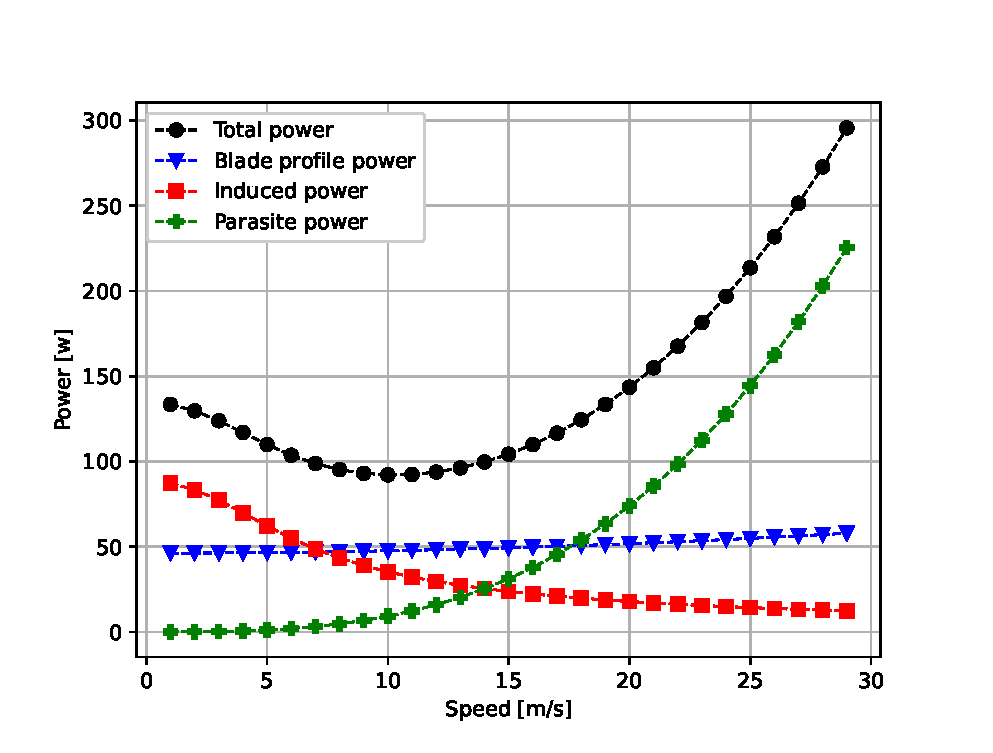
\includegraphics[width=0.55\textwidth]{Figures/speed_fig.eps}
    \vspace*{-5mm}
  \caption{Power consumption versus UAV speed.}\label{power_consum}
\end{figure}

\begin{equation}\label{total_power}
P_{total} = P_{blade} + P_{parasite} + P_{induced}
\end{equation}
where $P_{blade}$ is the power required to turn the rotors’ blade, and it is given by:
\begin{equation}\label{p_blade}
P_{blade} = K\left( 1 + 3\frac{v^2}{v_b^2}\right)
\end{equation}
where $v$ is the UAV velocity, $v_b$ is the blade’s rotor speed, and $K$ represents a constant which depends on the dimensions of the blade.

Parasite Power is the power used to overcome the drag force resulted from moving through the air.
\begin{equation}\label{parasite}
P_{parasite} = \frac{1}{2} {\rho{v}^3F}
\end{equation}
$\rho$ is the air density, and $F$ represents a constant that
depends on the UAV drag coefficient and reference area.
Note that this power is proportional to the UAV velocity $v$; it
is zero when hovering and gradually increases by the speed
of the UAV.

This power is required to lift the UAV and overcome the drag caused by the gravity. Whenever a UAV is moving, the airflow coming at it redirects the UAV and helps to lift it. Hence, the induced power has inverse proportion to the airspeed. When hovering, all the airflow needed to lift the UAV has to be created by the blade rotors, which results in more power consumption. The induced power can be written as follows:
\begin{equation}\label{induced}
P_{induced} = {m}{g}{v_i}
\end{equation}
where $m$ and $g$ respectively denote the mass of the UAV and the standard gravity, whereas, $v_i$ represents the mean propellers’ induced velocity in the forward flight, and it is given by:
\begin{equation}\label{v_i_power}
v_{i} = \sqrt{\frac{-{v^2}+\sqrt{v^4 + (\frac{mg}{A})^2}}{2}}
\end{equation}
with $A$ being the area of the UAV.
In the case of hovering, (i.e., when $v = 0$), the total power consumption is limited to hovering power and is calculated accordingly:
\begin{equation}\label{P_hover}
P_{total} = P_{hover} = K + \sqrt{\frac{(mg)^3}{2{\rho}A}}
\end{equation}

In Fig. \ref{power_consum}, we show the trend of the three power consumption factors as well as the total power versus the UAV speed. As it is shown in the figure, we can conclude that at optimal speed $(10 [m/s])$, the UAV consumes less power compared to hovering time. Thus, in order to minimize the localization error with the knowledge of limited UAV battery, it is not always desirable to increase the number of RSS samples.




\section{problem formulation}


In this work, we aim to maximize the number of transmitted bits and
minimize the localization error of ground users at the same time while taking in to account the constraint on UAV energy consumption. The UAV is required for perception of the urban environment and to implement real-time path planning. The decision of UAV flight trajectory and the choose of hovering position should consider the quality of communication, the precision of localization for ground users and energy consumption of UAV. As for the number of transmitted bits, its maximization depends on the amount of  data that are sent over the UAV mission period. It can be easily concluded that to maximize Rsum, on one hand, the UAV should fly at a lower speed so that it can have a higher flight time, which means more transmitted bits. On the other hand, the hovering location should be close to the target users so as to improve the data rate. From this aspect, hovering over the intersection of all users is the best choice. As for the minimization of localization error, besides the maximization of RSS samples, we hope that more samples are taken from different positions on the UAV. It may conflict with the UAV’s hovering directly over the intersection point of ground users to get the maximum data rate. As for the constraint of UAV’s energy consumption and flight time, it is clear that slower speed can achieve minimum energy consumption and higher flight time. However, it may be not fast enough to collect more RSS samples and reduce the localization error.

It is evident that these two objectives are in conflict with each other partially. Due to the random distribution of devices and their dynamic numbers, it is considerably complicated and may impose significant computational cost to identify an optimal trajectory and hovering location decision. Moreover, the environment is partly observed, traditional model-based methods like dynamic programming method are incapable to solve this problem. Recently, DRL has accomplished an excellent ability to solve complex problems and is considered as one of the core technologies of machine learning. With integration of deep learning and RL, it owns the strong understanding ability and decision-making ability and thus can realize end-to-end learning. It has shown great potential in solving sophisticated network optimizations. DDQN, which is one of the DRL algorithms, has been proved that can learn effective polices in problems with complex optimal policy in great state space. It is suitable for our proposed UAV’s flight decision problem where UAV is operating in a stochastic environment. Since the reward of original DDQN algorithm is scalar, we extend it to weighted sum reward for the multi objective optimization problem. The problem can be formulated as:


\footnotesize
\begin{IEEEeqnarray}{rCl}%notation is for 2D trajectories
\IEEEyesnumber\label{eq:both} \IEEEyessubnumber*
&& \underset{\mathbf{x,y,v}}{\text{max}} \left( W_{1} \mathbb{E}\sum_{k=1}^{K} R_n[k] + W_{2} MSE (\hat{x_k},\hat{y_k}), (x_k,y_k) \right) \forall k\\
\text{s.t.}
&& E_{total}[n] \leq \lambda B_{u}\\
&& l_{min} \leq x[n] \leq l_{max}, \,\  \forall n\\
&& l_{min} \leq y[n] \leq l_{max}, \,\  \forall n\\
&& v_{min} \leq v[n] \leq v_{max}, \,\  \forall n\\
&& z[n] = H_{u}, \,\  \forall n \\
&& P_{t}[n] = P_u, \,\  \forall n
\end{IEEEeqnarray}
\normalsize




In summary, we aim to find a control policy that can 1) maximize the system throughput; 2) minimize the localization error, and 3) ensure that the energy consumption of UAV does not exceed the battery capacity and the UAV is capable to return safely to recharging station. It is quite challenging to achieve all of these objectives because on one hand, to provide effective communication, it is preferred for the UAV to hover at a optimal position, one the other hand to minimize the localization error, it is preferred for the UAV to move around to different locations; and to minimize the energy consumption, it is preferred to reduce UAV movements (for energy savings). Hence, a good solution to this problem is supposed to well address this trade-off. Furthermore, (6.18b) ensures the UAV energy consumption to not exceed $\lambda$ percentage of UAV on-board battery, (6.18c), (6.18d) and (6.18e) indicates the boundary of horizontal movements and speed of UAV in the environment, respectively. Also, (6.18f) and (6.18g) set the constraints for UAV's altitude and transmit power, respectively. 








\section{Calculating localization error}

In this section, we clarify how the UAV estimates the location of ground users with received RSSI, and utilizing multilateration repeatedly to minimizes the average position errors. To be more specific, we will describe how to calculate $e[n]$ from reward function described in (\ref{reward_fun}) and estimate future Q-value function $Q(s_{t+1},a_{t+1})$ for RL agent. Here, we depicts the localization process for single user and then it can as well be applied to other users. Finally, the average localization errors from all users will be the measured metric for the RL reward and Q-value at each state.
In Fig. \ref{fig.fig_2}, we show the localization error reduction of a user by utilizing multilateration technique. The user to be located is highlighted by red dot, the UAV path by blue dashed lines, and user estimated location area by shaded green color. In the initial stage, by receiving RSSI measurement at on time stamp, following the channel model and (\ref{d_estimate_1}) in section \ref{sec_system}, the location of of the user is estimated in the shaded green zone between the inner ($I_1$) and outer ($O_1$) circles. The radius of these circles is dependent on the shadowing parameter and path loss exponent. In the next stage, when the UAV traverse to the next position and measure another RSSI measurement, the localization zone shrinks. Whenever the number of measurements becomes three, the position of the user can be estimated using trilateration, and consequently, the calculation of the localization error. As the number of samples and RSSI measurements increase, the localization error correspondingly reduces.

\begin{figure}[t!]
\vspace{-10pt}
  \centering
    %\vspace{-200pt}
  \includegraphics[width=0.55\textwidth]{Figures/fig2.pdf}
    \vspace*{-1mm}
  \caption{Tilateration for the case of one node in which shadowing component is bounded between two values.}\label{fig.fig_2}
\end{figure}




In Fig. \ref{fig.fig_2}, we illustrate how the error for one user using three samples can be calculated. The intersection point between three lines and connect inner and outer circles presents the estimated position of the user. Thus, the localization error can be obtained by finding the farthest border point to the estimated point as shown in the black line in the figure. Here, we consider the Cartesian coordinate for the estimated location of the user is $(\hat{x},\hat{y})$. Let $({x_s__i},{y_s__i})$ be the known ground position of the UAV at sample point $i$, and $\Bar{r_i} = \frac{O_{i} + I_{i}}{2}$ be the distance from sample point $i$ to the middle of the two circles, then the estimated position $(\hat{x},\hat{y})$ using $M$ number of samples can be calculated from the following optimization model:


\begin{equation}
(\hat{x},\hat{y}) = \underset{\hat{x},\hat{y}}{\operatorname{argmin}} \{ \sum_{i=1}^{M} \left( \sqrt{({x_s__i}-\hat{x})^2 +({y_s__i} - \hat{y})^2 } - \Bar{r_i}^2    \right)  \}
\end{equation}



The border points of the estimated zone of the user are generated each by the intersection of two RSSI circles. Fig. \ref{fig.fig_4} shows how a border point is found. As shown in the figure, $r_1$ and $r_2$ are respectively the radius of sample points $s_1$ and $s_2$, and $k$ is the distance between the two sample points. Moreover, $p_1$ and $p_2$ are the required intersection points between two circles, and $p_0$ is the intersection point of the perpendicular line connecting $p_1$ and $p_2$ with line $k$. Respectively, $q_1$ and $q_2$ denote the distances from $s_1$ to $p_0$, and from $p_0$ to $w_2$, respectively. Now, if we let $({x_s__1},{y_s__1})$, $({x_s__2},{y_s__2})$, $({x_p__0},{y_p__0})$,$({x_p__1},{y_p__1})$, and $({x_p__2},{y_p__2})$ define respectively the Cartesian coordinates for points $w_1$,$w_2$,$p_0$,$p_1$, and $p_2$, then the border points are calculated through the following equations:

\begin{equation}
%x_{P_1,P_2} = {x_{P__0}} \pm \frac{\left( {y_{s__2}}- {y_{s__1}} \right)}{k}
x_{p_1,p_2} = {x_{p_0}} \pm \frac{\left( {y_{s__2}}- {y_{s__1}} \right)}{k}
\end{equation}

\begin{equation}
y_{p_1,p_2} = {y_{p_0}} \mp \frac{\left( {x_s__2} - {x_s__1} \right)}{k}
\end{equation}


\begin{figure}[t]
\vspace{-10pt}
  \centering
    %\vspace{-200pt}
  \includegraphics[width=0.55\textwidth]{Figures/fig_4.pdf}
    \vspace*{-1mm}
  \caption{Illustration of attaining the intersection point between two RSSI arcs.}\label{fig.fig_4}
\end{figure}

where $({x_p__0},{y_p__0}) = (x_{s1} + \frac{(x_{s2}-x_{s1})q_{1}}{k}) , (y_{s1} + \frac{(y_{s2}-y_{s1})q_{1}}{k})$ , $q_1 = \frac{r_1^2 - r_2^2 + k^2}{2k}$ and $h = \sqrt{r_1^2 - q_1^2}$.
After a new RSSI sample received by the UAV, the accuracy of the estimated user localization zone is updated by first removing the the previous border points and then add new intersection points (described above) and finally find distances from all obtained zone points to the estimated user point, and the one with farthest distance is the user's localization error. After obtaining the localization error for all ground users in the current state $s_t$, we average over all error values. Then, we evaluate the reward function corresponding to localization in eq. (\ref{reward_fun}) by dividing the localization error calculated in the current state by $e_{min}$ which is the set to arbitrary value for minimum possible localization error, i.e $10[m]$. Similarly, we estimate the future average localization errors for all available neighbor sample points and actions, and we update the approximated Q-value function for all actions and store them into the table. Subsequently, for the next iteration, we choose the action that results in higher reward by looking at the stored Q-value functions.





\section{preliminaries}


As shown in Fig. 1, utilizing the multilateration technique to find the position of targets with lower localization errors, the UAV needs to travel to more waypoints. However, with limited flight time due to the UAV battery capacity and the path length, a certain UAV trajectory results in optimal localization precision. Therefore, to find the best trajectory, we let the UAV interact and observe the environment by using RL and learn to autonomously find the optimal trajectory that can achieves the minimum localization errors. In this section, we review the RL framework, a machine learning approach which is suitable for controlling an autonomous machine such as UAV.

RL is a learning approach that is used for finding the optimal way of executing a task by letting an entity, named agent, take actions that affect its state within the acting environment. In RL, the environment is typically formulated as an MDP, which is described by four tuples ($S$,$A$,$R$,$P$), set of possible state $S$, set of available actions $A$, and reward function $R: S{\times} A $ and transition probability $P(\hat{s} | s,a) \rightarrow [0,1] $. The agent interacts with an unknown environment through the repeated observations, actions, and rewards to construct the optimal strategy. When interacting with the environment, after choosing an action $a_t \in A$, the agent receives a reward $r(s_{t},a_{t})$ and moves to the next state $s_{t+1}$. The goal of RL is to learn from the transition tuple , and find an optimal policy $\pi^*$ that will maximize the cumulative sum of all future rewards. Note that the policy $\pi = \left({a_{1},a_{1},...,a_{T}\right)$ defines which action $a_t$ should be applied at state $s_t$. If we let $r\left(s_{t},\pi(a_t)\right)$ denote the reward obtained by choosing policy $\pi$, the cumulative discount sum of all future rewards using policy $\pi$ is given by:

\begin{equation}
R_{\pi} = \sum \gamma^{t-1} r(\left s_{t}, \pi(a_t)\right)
\end{equation}
where $\gamma \in [0,1)$ is a discount factor, which measures the weight given to the future rewards (i.e., when $\gamma =0$, the agent considers only the current received rewards, whereas, when the factor approaches one, the agent strives for future higher reward). Now, let $\Lambda$ denote the set of all admissible policies. Then, the optimal policy is given by:

\begin{equation}
\pi^* = \underset{\pi \in \Lambda}{\operatorname{argmax}} R_{\pi}
\end{equation}
Note that RL is modeled as a Markov Decision Process (MDP), where the tuple $(s_{t},a_{t},r(s_{t},a_{t}),s_{t+1})$ is conditionally independent of all previous states and actions. Therefore, the agent does not need to memorize or save all the state-action tuples, just the last one, and subsequently updates it at each cycle or iteration.

In this work, we rely on double-Q-learning algorithm to solve our problem which allows us to keep two separate agents with the same properties but with different weight values $w_P$ and $w_T$ . As such they will output a different Q-action function when given the same state. One is used to choose the actions, called a primary model $\textit{Q}_{P}(s_t, a_t)$, while the other model evaluates the action during the training, called a target model $\textit{Q}_{T}(s_t, a_t)$. Therefore training occurs when taking a batch of experiences $e_t$ from the buffer that is used to update the model as:
\begin{equation}\label{Double-dqn}
\textit{Q}_P^{new} = (1 - \alpha)\textit{Q}_p + \alpha \left[r_t + (1-d_t)\gamma \max{\textit{Q}_T(s_{t+1},a)} \right]
\end{equation}
where $\max{\textit{Q}_T(s_{t+1},a)}$ is the action chosen as per the agent, $\alpha$ is the learning rate which was an input to the Adam optimizer \cite{kingma2014adam}, and $\gamma$ is a discount factor that reduces the impact of long term rewards. We implement this with soft updates where instead of waiting several episodes to replace the target model with the primary. The target model receives continuous updates discounted by value $\tau$ as in $w_T = w_T(1 - \tau) + w_P\tau$.



\floatstyle{plaintop}
\restylefloat{table}

\begin{table}[t]
\begin{center}
\begin{tabular}{ | m{5.75cm} | m{2cm} | }
 \hline
   UAV's altitude $(h)$ & $100 [m]$ \\
  \hline
   Rotor solidity $(s)$ & $0.05$ \\ 
   \hline

   Profile drag coefficient $(\delta)$  & $0.012$ \\ 
   \hline
   
   UAV weight $(N)$ & $20[N]$\\ 
   \hline
 
   Air density $(\rho)$ & $1.225 [kg/m^3]$  \\ 
  \hline
   
   Rotor disc area $(A)$  & $0.503 [m^2]$ \\ 
   \hline
   
   Rotor blade tip speed $(U_{tip})$ & $120 [m/s]$  \\ 
   \hline
   Induced power correction factor $(k)$ & 0.1 \\ 
   \hline
   Environment constant for $P_{LoS}$ ($a_0$)  & $45$ \\ 
   \hline
 Environment constant for $P_{LoS}$ ($b_0$)  & $10$ \\ 
   \hline
  Shadowing constant for $P_{LoS}$ $(a_{LoS})$  & $10$ \\ 
   \hline
  Shadowing constant for $P_{LoS}$ $(b_{LoS})$  & $2$ \\ 
   \hline
   Shadowing constant for $P_{NLoS}$ $(a_{NLoS})$ & $30$ \\
   \hline
   Shadowing constant for $P_{NLoS}$ $(b_{NLoS})$ & $1.7$ \\ 
   \hline

\end{tabular}
\caption{Simulation Parameters}
\label{table_env}
\end{center}
\end{table}

\floatstyle{plaintop}
\restylefloat{table}

\begin{table}[t]
\begin{center}
\begin{tabular}{  m{4cm} m{4cm}  }
 \hline
 \hline
   \textbf{Parameters}  & \textbf{Values}\\ 
 \hline
   Number of training episodes & $16000$ \\ 
 
   Learning rate & $0.0001$ \\ 
 
   Discount factor & $0.99$\\ 
   
   Replay memory size & $8000$\\ 
 
   Batch size & $32$  \\ 
   
   Number of neurons & $256$  \\ 
   
   SGD optimizer & Adam  \\ 
   
   Activation function & ReLU  \\ 
   \hline
   \hline
 
\end{tabular}
\caption{Network Configuration}
\label{table_env}
\end{center}
\end{table}


\begin{figure}
\vspace{-10pt}
\hspace*{-0.2in}
  \centering
   %vspace{-5pt}
  \includegraphics[width=0.55\textwidth]{Figures/my_figure_6.pdf}
    \vspace*{-5mm}
  \caption{Accumulated reward vs number of training episodes.}\label{Results_1}
\end{figure}

\subsection{Proposed RL framework}

It is of great importance to cast the optimization problem into the MDP in a proper way. The agent rely on the interaction with the environment to adapt its behavior and learn optimal policies. In the following, we present a detailed description of state space, action space and reward in our model.

1) State Space: Collecting the real-time parameters in the environment depends on frequent information exchange between the UAV and ground devices. This will cause delay, considerably reducing the efficiency of the system and occupy a large amount of wireless resources. To be more realistic, we consider that the UAV can only observe its own state and partial network information. Specifically, UAV can record its own location, the estimated distances and localization error of ground targets, communication rate of users and UAV energy consumption. Thus the state space is defined symbolically as:

\begin{equation}
\textit{S} = \{\textbf{s}_t\} = \{ x_{u}(t),y_{u}(t) , d_{j}(t), e_{j}(t), R_{k}(t), E_{u}(t)   \}
\end{equation}
where $d_{j}(t)$ is the distance between the target device and the UAV under the Cartesian coordinates, $e_{j}(t)$ is the calculated localization error described in previous section, $R_{k}(t)$ is the communication rate of the corresponding user and $E_{u}(t)$ is the energy consumption of the UAV . In practical scenarios, most of the information is not necessary for decision-making. In our setup, we extract a small amount of essential information to represent the state of the environment. These elements of state space will enable the UAV to have a reasonable general perception of the environment. Moreover, it overcomes the lack of network information which is common problem that exists in DFRC systems.

%2) Action Space: The action space $A$ is described by all possible movement directions and the action of remaining in the same place. By assuming that the UAV fly with simple coordinate turns, the actions related to movement of UAV is simplified to $7$ directions.

2) Action Space: When the UAV is operating in the environment and observes a state, it makes action decision in real time. The action space can be defined as:
\begin{equation}
\textit{A} = \{\textbf{a}_{t}\} = \{ [v(t)\cos{\theta (t)}, v(t)\sin{\theta(t)}] \}
\end{equation}
We utilize $[\cos{\theta} (t), \sin{\theta(t)}]$ to depict yaw and then the network will learn a normalized two-dimensional vector. The flying speed of the UAV $v(t)$ and the yaw Angle $\theta(t)$ are assumed to be discrete values in the interval $[0, v_{max}]$ and $[{-}\pi, \pi]$, respectively.


3) Reward: The reward function incorporates instantaneous throughput of users and localization error of targets. It can be written as follows:
\begin{equation}\label{reward_fun}
r[n] = {w_{R}} \frac{R_{max}}{R[n]} + {w_{L}} \frac{e_{min}}{e[n]}
\end{equation}
where $R_{max}$ is the maximum achievable rate in the environment, $e_{min}$ is minimum desired localization error, $w_R$ and $w_L$ are corresponding weights for each reward function.












\begin{figure*}
\captionsetup{justification=centering}
        \begin{subfigure}[b]{0.33\textwidth}
                \centering
                \includegraphics[width=1\linewidth]{Figures/my_figure_1.eps}
                \caption{}
                \label{fig.1a}
        \end{subfigure}%
        \begin{subfigure}[b]{0.33\textwidth}
                \centering
                \includegraphics[width=1\linewidth]{Figures/my_figure_2.eps}
                \caption{}
                \label{fig.1b}
        \end{subfigure}%
        \begin{subfigure}[b]{0.33\textwidth}
                \centering
                \includegraphics[width=1\linewidth]{Figures/my_figure_4.eps}
                \caption{}
                \label{fig.1c}
        \end{subfigure}
        \caption{Training curves tracking optimization objectives: (a) Number of transmitted bits; (b) Localization error; (c) UAV flight time.}\label{fig_FL}
\end{figure*}


\begin{figure*}
\begin{center}
\captionsetup{justification=centering}
        \begin{subfigure}[b]{0.33\textwidth}
                \centering
                \includegraphics[width=1\linewidth]{Figures/new_fig_1.eps}
                \caption{}
                \label{fig.2a}
        \end{subfigure}%
        \begin{subfigure}[b]{0.33\textwidth}
                \centering
                \includegraphics[width=1\linewidth]{Figures/new_fig_2.eps}
                \caption{}
                \label{fig.2b}
        \end{subfigure}%
        \caption{Impact of UAV speed on (a) Number of transmitted bits and localization error; (b) UAV flight time.}\label{fig.2}
\end{center}
\end{figure*}


\section{Simulation Results}

In this section, we evaluate the performance of our RL approach in localizing terrestrial targets and giving service to ground users numerically. We generate randomly the locations of the targets and ground users, in which we want the UAV to localize and giving service communication, respectively. Based on the environment parameters  and the probability of LoS, we evaluate the range between the inner-circle and outer-circle where the target is located from the ground reflection of UAV’s position. Thus, the zone attained from the intersection of multiple inner and outer circles  is considered as the location zone of the target. Consequently, the localization error or accuracy can be evaluated by calculating the distance from the farthest border point to the center of the zone. Moreover, by adding more samples from different positions, the location error is reduced.

\begin{figure*}[t]
%\multifig% better safe than sorry
\centering
\begin{tabular}{ccc}
%\figtarget & \figtarget & \figtarget \\
%Speed =10 & Speed =20 & Speed =30 \\
\includegraphics[width=2in]{Figures/10_w_1.eps} & 
\includegraphics[width=2in]{Figures/20_w_1.eps} &
\includegraphics[width=2in]{Figures/30_w_1.eps} \\
%\figcaption{first} & \figcaption{second} & \figcaption{third} \\
%\figtarget & \figtarget & \figtarget \\

\includegraphics[width=2in]{Figures/10_w_2.eps} &
\includegraphics[width=2in]{Figures/20_w_2.eps} &
\includegraphics[width=2in]{Figures/30_w_2.eps}\\

\includegraphics[width=2in]{Figures/10_w_3.eps} &
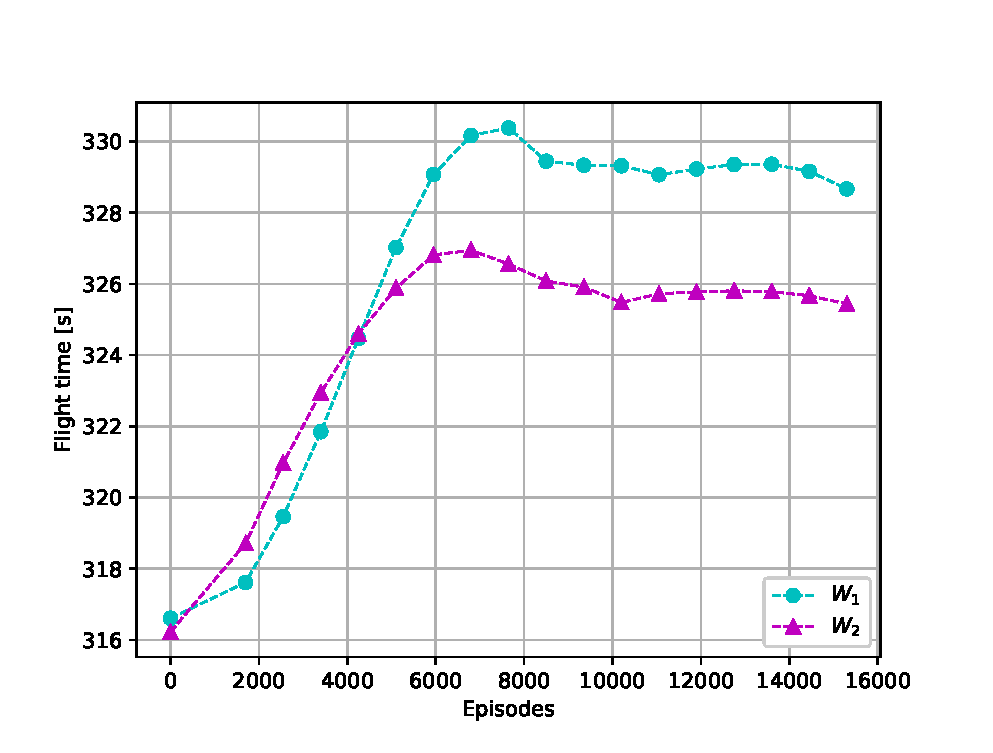
\includegraphics[width=2in]{Figures/20_w_3.eps} &
\includegraphics[width=2in]{Figures/30_w_3.eps}\\
(a) Speed = 10 [m/s]  & (b) Speed = 20 [m/s] & (c) Speed = 30 [m/s] \\

%\figcaption{fourth} & \figcaption{fifth} & \figcaption{sixth}
\end{tabular}
\caption{Performance comparison for two sets of weights in (\ref{reward_fun}).} \label{Results_4}
\end{figure*}



For the numerical study, we assume $10$ terrestrial targets and $20$ ground users which are randomly distributed in a region of $750 \times 750 \ m^2$. We also assume the UAV is flying at a fixed altitude $H_u$. The parameters used in this section and their corresponding values (taken and recommended by [5], [28], [30], [38] for urban environments) are listed in Table 1. In summary, we first illustrate the convergence of the proposed DDQN in the considered multi objective optimization problem. Then we study the performance of our system for communication and sensing  by varying UAV’s speed. Later on, we study the performance of our RL method by varying the corresponding weights for communication rate and localization error in our RL reward function. Finally, we show the performance trade-off between localization error and number of transmitted bits.



%\lipsum[1-10]




We start by illustrating the effectiveness and convergence of the proposed DDQN algorithm. The learning curve of the trained DDQN agent is shown in Fig. \ref{Results_1}. The figure plots the accumulated reward versus number of training episodes. Here, the weight parameters are set to $W_R = W_L = 1.0$. We consider the jointly optimization of two objectives. It can be seen in Fig. \ref{Results_5} that the agent quickly learns to obtain higher expected total rewards as training progresses. And then the accumulated reward converges steadily at a high level. At first about $10000$ episodes, the accumulated reward fluctuates at a very low level. It is because that the UAV is in complete experience stage. Without enough experience to learn from, the action is chosen randomly. At the same time, the loss of the network is 0 and the objectives are not optimized. When the replay memory is full, the UAV begins to sample the stored experience tuples to train networks. We can see that there is a major exploration and learning stage before about
the $10000$th episode.

%During this stage, the loss of network drops rapidly after a sharp rise. Within the same period, the sum data rate as well as total harvested energy increase rapidly while energy consumption is reduced

The changing trend of two objectives as well as flight duration of corresponding results during the training are also illustrated in Fig. \ref{fig.1a}, Fig. \ref{fig.1b} and Fig. \ref{fig.1c}. We start by examining the results obtained by training the RL agent and compare different UAV speeds on localization and communication performance. Fig. \ref{fig.1a} depicts the number of transmitted bits achieve during multiple episodes for training RL agent. As it is shown in the figure, after $8000$ episodes the RL agent reaches convergence. As can be seen in the figure, the UAV operating at speed $30 [m/s]$ can transmit around $330$ bits, while moving at speed $20 [m/s]$ it can transmit approximately $360$ bits and when traversing with $10 [m/s]$, the UAV can transmit $400$ bits during its mission duration. Fig. \ref{fig.1b} illustrates the localization error obtained through training episodes. We can observe that after $8000$ episodes, the RL agent reaches convergence for minimizing localization error. As the figure shows, when UAV is moving at speed $30 [m/s]$, it can achieve the localization error of $28 [m]$ while moving at speed $ [m/s]$, it can reach the localization error of $34$ and when the UAV is operating with $10 [m/s]$, it achieves $40 [m]$ error for localization. In the Fig. \ref{fig.1c}, we show the flight time of UAV during training. Similar to previous figures, the UAV will return back to recharging station after reaching $70\%$ of its battery and the RL agent reaches the convergence after $8000$ episodes. From the figure we can see that the UAV has a flight time of $360$, $330$ and $320 [s]$ when moving at speed $10$,$20$ and $30$ $[m/s]$, respectively.


%sufficient training episodes, UAV at speed $30$ performs worst and attains the lowest amount of transmitted bits during the given period of time and for the best case, UAV at speed $10 m/s$ achieves the highest transmitted bits. Fig. \ref{Results_2} illustrates the localization error obtained through training episodes. We can see that after the training converges, the UAV at speed $10 m/s$ performs worst in comparison with other UAV speed's and at $30 m/s$, it achieves the best performance by reaching the localization error of $30 m$.


%the flight time of UAV at speed $30$ is lowest, speed $20$ is the second lowest and speed $10$ is the highest. This trend is evident as discussed in Fig. \ref{label-speed-source}, in which the energy consumption of UAV rises as the UAV speed increases. With respect to Fig. \ref{Results_1}, Fig. \ref{Results_2} and Fig. \ref{Results_3}, the relation between UAV speed, number of transmitted bits and localization error become clear. 

%It can be seen that when the UAV operates at speed $10$, since it consumes less energy than other speed variations and the flight time is the highest, thus it can achieve the highest number of transmitted bits. On the other hand, when the UAV move at speed $30$, it consumes the highest energy and so lowest flight time and low number of transmitted bits. However, since it is moving at higher speed, it travels the longest path which means RSSI samples from different positions that results to better localization error. From the figures, it is clear that with limited energy the localization error reduces along with increasing the UAV speed, but the number of transmitted bits lessened.

%talk about the flight time figure and why the figures are decreasing or increasing for different speeds%







Fig. \ref{fig.2} summarizes the comparison results for UAV speed on three performance metrics. The UAV speed is set from $10 m$ to $40 m$. It can be seen that when the UAV operates at lower speeds, since it consumes less energy than other speed variations and the flight time is the highest, it can achieve the highest number of transmitted bits. On the other hand, when the UAV move at  higher speeds, it consumes the largest energy based on the adopted propulsion power consumption model and so lowest flight time and low number of transmitted bits. However, since it is moving at higher speed, it travels the longest path which means RSSI samples from different positions that results to better localization error. From the figures, it is clear that with limited energy the localization error reduces along with increasing the UAV speed, but the number of transmitted bits lessened.




In Fig. \ref{Results_4}, we evaluate the performance of RL approach by varying the weights in the reward function from (\ref{reward_fun}). For this purpose, we tested different weight numbers for communication rate and localization error rewards. Here, we chose two set of weights values ($W_1$ and $W_2$) that can capture the impact of reward function in the trade-off between communication and localization. $W_1$ corresponds to the scenario when the weight of the communication reward is larger than localization, and $W_2$ is for the case in which the weight of the localization is larger than communication. Figure. 7a plot the number of transmitted  signals, localization error and flight time during each training session when the uav speed is set to $10 [m/s]$. It can be seen that for the case of $W_1$, after convergence, the UAV achieves higher transmitted bits during an episode in comparison with $W_2$. However, in $W_2$ case, the UAV archives better localization performance than $W_1$. The flight time difference between these two cases capture the fact that when weight for communication reward is larger than localization reward, the UAV tends to hover more than moving to different spots which means that the UAV found the optimal spot for giving service to ground users and hover at that position to maximize the system throughput.


\begin{figure}
\vspace{-20pt}
\hspace*{-0.2in}
  \centering
   %vspace{-5pt}
  \includegraphics[width=0.55\textwidth]{Figures/my_figure_5.eps}
    \vspace*{-5mm}
  \caption{Localization error versus number of transmitted bits.}\label{Results_5}
\end{figure}


In Fig. \ref{Results_5}, we show the trade-off between communication and sensing with respect to discussion in previous sections on multi objective optimization of localization and system throughput. The figure plots the localization error and number of transmitted bits resulted from different UAV speeds and multi objective weights in (\ref{reward_fun}). In fact, whenever we increase the transmitted bits, the localization error decreases. Thus, we can see the trade-off between these two optimization objectives. To achieve any  specific system performance, we can modify the weight values $W_R$ and $W_L$ in (\ref{reward_fun}) and UAV speed to achieve desirable communication throughput and localization error.




\section{Conclusion}

In this paper, we studied a multi objective optimization for UAV path planing in a DFRC network, where a single UAV is employed to simultaneously serve a group of ground users for communications and localize the ground targets. Averaged number of transmitted bits as well as localization error  were optimized simultaneously. Since the UAV communication channel was uncertain and dynamic due to the environment path loss, we proposed a novel framework using DDQN to achieve online control of the UAV. The reward function was designed as a function corresponding to the optimization objectives. Thus the UAV learns to find the trajectory optimization solution according to weights parameters associated with the objectives. Simulation results showed the validity of our approach and proved that the model can produce optimized policies under different weights. In addition, it has been shown that the UAV equipped with DFRC has great advantages in completing complex tasks through  training in the unknown environment. Thus, it is worthy of studying the cooperative objective and resource management and multi-UAV path planning for UAV swarm as DFRC network in the future.





\bibliographystyle{ieeetr}
\bibliography{ref}

\end{document}
